% ---------------------------------------------------------------------------
% ICCE-Asia 2026 submission. The conference's submission page states 2--6
% pages, two-column, at least 10pt, on A4 -- hence a4paper below, which
% IEEEtran does not default to. Blinding is still unconfirmed, and this file
% has never been built against the venue's own template package
% (see paper/README.md).
%
% Numbers are never typed into prose by hand. Tables are \input from the
% directories the harness writes; prose figures come from macros in
% numbers.tex, which names the single run each one was measured in. If a
% measurement is re-run, numbers.tex is the one file that changes.
% ---------------------------------------------------------------------------
\documentclass[conference,a4paper]{IEEEtran}
\IEEEoverridecommandlockouts

\usepackage{cite}
\usepackage{amsmath,amssymb}
\usepackage{graphicx}
\usepackage{booktabs}
\usepackage{url}
\usepackage[hidelinks]{hyperref}

% ---------------------------------------------------------------------------
% Every number that appears in prose, in one place, each tagged with the run it
% was read from. Nothing here is typed from memory; each value comes out of the
% JSON the harness wrote.
%
% All values are now FINAL: every experiment has been run at the scale the
% paper reports. The pilot-scale block at the bottom is kept only for the
% sentence that compares the two, and is labelled as such.
% ---------------------------------------------------------------------------

% --- E1: LEVIR-CD test, 128 tiles -- results/levir_cd_test/ ----------------
\newcommand{\EOnePixelFOne}{54.01}
\newcommand{\EOneIoU}{36.99}
\newcommand{\EOneInstFOne}{54.28}
\newcommand{\EOneHeuristicFOne}{25.59}
\newcommand{\EOneGeoFOne}{23.47}
\newcommand{\EOneNoVerifierFOne}{21.48}
\newcommand{\EOneCrossFrameGain}{4.71}
\newcommand{\EOneCrossFrameInstGain}{3.72}
\newcommand{\EOneGTDensity}{54.5}

% --- E2: WHU-CD test, 690 pairs -- results/whu_cd_test/ --------------------
% Re-measured on 2026-08-31 in one run that also produces the cross-frame
% ablation row the original E2 run omitted. geo-only, the heuristic and the
% greedy arm reproduce the earlier run exactly; the two Hungarian arms move
% (ours 57.92 -> 57.97, no-verifier 19.78 -> 20.84) because Hungarian
% assignment breaks ties non-deterministically. One run is quoted rather
% than two so the table has a single provenance.
\newcommand{\ETwoPixelFOne}{57.97}
\newcommand{\ETwoIoU}{40.82}
\newcommand{\ETwoInstFOne}{52.22}
\newcommand{\ETwoHeuristicFOne}{28.86}
\newcommand{\ETwoHeuristicInstFOne}{9.06}
\newcommand{\ETwoGeoFOne}{30.16}
\newcommand{\ETwoNoVerifierFOne}{20.84}
\newcommand{\ETwoCountMAE}{1.3}
\newcommand{\ETwoHeuristicCountMAE}{14.8}
\newcommand{\ETwoNPred}{1{,}426}
\newcommand{\ETwoHeuristicNPred}{11{,}204}
\newcommand{\ETwoNGT}{987}
\newcommand{\ETwoGTDensity}{1.4}
\newcommand{\ETwoCrossFrameGain}{9.82}   % 57.97 - 48.15 pixel F1
\newcommand{\ETwoCrossFrameInstGain}{4.24} % 52.22 - 47.98 instance F1

% --- Published zero-shot peer (AnyChange, LEVIR-CD) -- baselines.json ------
\newcommand{\AnyChangeFOne}{23.40}
\newcommand{\AnyChangeHFOne}{42.20}

% --- E3/E4: grounding ladder, 1929 crops -- results/levir_cc_caption/ ------
% vlm_direct merged in from results/levir_cc_caption_vlm (Qwen pass).
\newcommand{\EFourNCrops}{1929}
\newcommand{\EFourTemplateFOne}{48.20}
\newcommand{\EFourTemplateHal}{38.45}
\newcommand{\EFourRawFOne}{45.28}
\newcommand{\EFourStructFOne}{48.37}
\newcommand{\EFourFlatRagFOne}{48.51}
\newcommand{\EFourGraphRAGFOne}{48.32}
\newcommand{\EFourAggGain}{3.1}       % llm_raw -> llm_struct
\newcommand{\EFourLadderSpread}{0.2}  % struct / flat_rag / graphrag spread
\newcommand{\EFourStructChgAcc}{76.5}
% The external baseline.
\newcommand{\EFourVLMFOne}{28.49}
\newcommand{\EFourVLMChgAcc}{45.78}
\newcommand{\EFourVLMHal}{65.03}
\newcommand{\EFourVLMBleu}{4.51}
\newcommand{\EFourVLMGap}{19.83}      % llm_graphrag - vlm_direct, CFS-F1
% Over-assertion on crops the references call unchanged. Counted directly from
% the generation dumps against LevirCCcaptions.json: a crop is unchanged when at
% least three of its five references say so, and a report asserts change when it
% carries no no-change phrasing.
\newcommand{\EFourNNoChange}{965}
\newcommand{\EFourVLMFalseChange}{98.0}
\newcommand{\EFourGraphRAGFalseChange}{26.7}

% How much of the retrieval/graph difference reaches a claim.
\newcommand{\EFourTextDiffer}{1{,}313}
\newcommand{\EFourTextDifferPct}{68.1}
\newcommand{\EFourClaimsDiffer}{26}
\newcommand{\EFourClaimsDifferPct}{1.3}

% --- E5: pairing swapped, grounding fixed at llm_graphrag ------------------
% learned arm: results/levir_cc_caption (llm_graphrag row)
% heuristic arm: results/levir_cc_caption_heuristic_pairing
\newcommand{\EFiveLearnedFOne}{48.32}
\newcommand{\EFiveHeuristicFOne}{35.35}
\newcommand{\EFiveGain}{12.97}
\newcommand{\EFiveLearnedHal}{38.28}
\newcommand{\EFiveHeuristicHal}{65.99}
\newcommand{\EFiveLearnedChgAcc}{76.52}
\newcommand{\EFiveHeuristicChgAcc}{65.01}

% --- E6: deployment cost -- results/efficiency/ ---------------------------
% 512 pairs of the full LEVIR-CC cache. Two runs over that cache agree to
% 0.08 ms on the delta (0.62 at n=64, 0.70 at n=512); the 1.45 ms reported
% earlier came from the pilot cache, whose crops carry different detection
% counts -- a different measurement, not a noisier one.
% Quoted to three decimals so the difference reconciles with the two values it
% is derived from: 9.688 - 8.984 = 0.704. At two decimals a reader subtracting
% the printed numbers gets 0.71 and the quoted delta reads as an error.
\newcommand{\ESixHeadDelta}{0.70}
\newcommand{\ESixHeadMs}{9.688}
\newcommand{\ESixHeuristicMs}{8.984}
\newcommand{\ESixDetectMs}{6{,}099}
\newcommand{\ESixDetectShare}{91}
\newcommand{\ESixPipelineShare}{0.01}

% --- E7: neighbourhood level, 218 scenes -- results/levir_cc_scene/ --------
% Learned head; the checkpoint is recorded in the JSON.
\newcommand{\ESevenNScenes}{218}
\newcommand{\ESevenNMultiCrop}{129}
\newcommand{\ESevenMeanCrops}{8.8}
\newcommand{\ESevenMeanGT}{37.7}
\newcommand{\ESevenTemplateFOne}{40.99}
\newcommand{\ESevenStructFOne}{21.02}
\newcommand{\ESevenFlatFOne}{18.54}
\newcommand{\ESevenGraphFOne}{27.55}
\newcommand{\ESevenTemplateCountMAE}{26.15}
\newcommand{\ESevenStructCountMAE}{458.46}
\newcommand{\ESevenFlatCountMAE}{167.87}
\newcommand{\ESevenGraphCountMAE}{18.50}

% --- Pilot-scale values, kept only for the comparison sentence ------------
% 128 crops of the 8 largest scenes -- a favourable slice, which is why the
% full-scale numbers are lower. Do not typeset these as results.
\newcommand{\PilotEFourGraphRAGFOne}{54.64}
\newcommand{\PilotEFiveGain}{21.02}
\newcommand{\PilotESevenNScenes}{8}
\newcommand{\PilotESevenGraphFOne}{32.43}
\newcommand{\PilotESevenStructFOne}{35.14}

% --- Model / system constants ---------------------------------------------
\newcommand{\HeadParams}{19{,}781}
\newcommand{\HeadParamsRound}{20k}
\newcommand{\NPairFeatures}{16}
\newcommand{\NUnaryFeatures}{14}
\newcommand{\NCrossFrameFeatures}{4}
\newcommand{\LLMName}{EXAONE-4.0-32B}
\newcommand{\VLMName}{Qwen2.5-VL-7B-Instruct}
\newcommand{\DetectorName}{SAM3}


\begin{document}

\title{Grounding LLM Change Reports in Foundation-Model\\Instance Evidence for
Consumer Satellite Monitoring}

% TODO non-blind: fill in before submission.
\author{\IEEEauthorblockN{Author Name}
\IEEEauthorblockA{Affiliation\\
Email: songjae7175@gmail.com}}

\maketitle

\begin{abstract}
We build a satellite change-monitoring service for consumers --- a subscriber
pins a neighbourhood and, after each revisit, receives a short written report of
what changed --- from the current AI stack: a promptable segmentation
foundation model (\DetectorName) for open-vocabulary instance detection, CLIP
embeddings for appearance, a spatio-temporal knowledge graph for history, and a
large language model (\LLMName) for the report. Because the deliverable is
prose, we evaluate what it writes, not only what it segments. Two failures that
segmentation metrics cannot see become product failures: a report that invents
construction, and one that miscounts it. Neither is fixed where practitioners
reach first. Adding retrieval or graph aggregation to the language model's
context leaves factuality essentially unchanged; what moves it is the upstream
decision of which detections across two revisits are the same physical object.
A \HeadParamsRound-parameter pairing head, supervised for free from
change-detection masks, reaches \EOnePixelFOne{} pixel F1 on LEVIR-CD against
\AnyChangeFOne{} for the strongest zero-shot peer, and transfers to WHU-CD
unchanged at \ETwoPixelFOne. To measure reports we introduce Change-Fact-Score,
which reduces a report to atomic claims with a deterministic extractor, so no
language model sits inside the metric. It exposes what n-gram overlap hides: a
vision--language model shown both images writes fluent prose while deciding at
chance (\EFourVLMChgAcc\%) whether anything changed. Swapping only the pairing
moves report factuality by \EFiveGain{} points, at \ESixHeadDelta~ms per tile.

\end{abstract}

\begin{IEEEkeywords}
large language models, foundation models, vision--language models, change
detection, retrieval-augmented generation, knowledge graph, hallucination,
consumer services
\end{IEEEkeywords}

\section{Introduction}

We consider a change-monitoring application that turns repeated overhead
imagery into a consumer-facing subscription rather than an analyst-facing
mask: a homeowner watching the plot next door, a
small builder tracking three sites, someone deciding whether a district is
being built up or emptied out. Each pins an area in an app and, after every
revisit, receives a short message --- \emph{four new buildings on the north
edge; the lot behind the school has been cleared}. Nobody in this audience
wants a segmentation mask, and nobody will open one.

That shift changes which errors matter, in a way segmentation metrics cannot
express. The deliverable is a sentence, and a sentence makes commitments a mask
does not: it says \emph{how many} buildings appeared, and \emph{whether}
anything appeared at all. Two product failures follow.

\begin{enumerate}
\item \textbf{Invention.} A report announcing construction that never happened
      is worse than no report: the subscriber walks out to look, finds nothing,
      and stops trusting the service. Pixel precision cannot see this, because
      it is computed against a mask the user never sees.
\item \textbf{Miscounting.} ``Several buildings appeared'' when the answer is
      one is directionally correct and operationally useless. A model can score
      well on IoU while the instance count derived from it is off by an order of
      magnitude, because IoU rewards covering the right pixels rather than
      resolving the right objects.
\end{enumerate}

\textbf{A direct vision--language baseline fails on both.} A practitioner asked to ship this
today would hand both images to a vision--language model and ask for a
description. We measure that baseline rather than dismiss it: it writes fluent,
confident prose while reaching only \EFourVLMChgAcc\% accuracy on whether the
scene changed. Its BLEU-4 is
\EFourVLMBleu, which reads as a stylistic mismatch rather than as the symptom
it is. Such a service would look correct in demos while remaining unreliable
in many evaluated cases.

\textbf{Our approach} grounds the text in explicit instance evidence.
\DetectorName~\cite{sam3} proposes object instances in each frame
open-vocabulary, without having been trained on either benchmark;
CLIP~\cite{radford2021learning} embeddings describe appearance; a learned head
decides which detections across revisits are the same object and which
unmatched detections are genuine change; survivors accumulate in a
spatio-temporal knowledge graph keyed by location; and
\LLMName~\cite{exaone4} writes the report from that structure rather than from
pixels. Because the report is assembled from objects, counting is a property of
the evidence rather than of the prose.

\textbf{Where factuality is won was not where we expected.} The
retrieval-augmented generation literature encourages the assumption that the
language model's context is the lever. Over \EFourNCrops{} crops we find
otherwise: aggregating raw detections into a change inventory is worth
\EFourAggGain{} CFS-F1, but adding top-$k$ retrieval or graph aggregation on
top moves factuality by less than \EFourLadderSpread{} points, in both
directions. What moves it, by \EFiveGain{} points, is improving the pairing
that produced the evidence. The design implication is direct: spend the
engineering budget upstream of the language model, not on its prompt.

Our contributions are as follows.

\begin{itemize}
\item An LLM change-reporting pipeline built on segmentation and
      vision--language foundation models, evaluated on the factuality of its
      prose rather than only on segmentation overlap.
\item \textbf{Learned instance pairing.} Every non-learned strategy we tested
      --- geometry, a hand-tuned CLIP-plus-geometry heuristic, and the
      published zero-shot reference --- lands in the same narrow band
      (\EOneGeoFOne, \EOneHeuristicFOne, \AnyChangeFOne{} F1) regardless of
      segmentation quality, although the supervision settings differ. A
      \HeadParamsRound-parameter head trained without additional correspondence
      annotations leaves it at
      \EOnePixelFOne{} and transfers to WHU-CD unchanged at \ETwoPixelFOne,
      cutting instance count error from \ETwoHeuristicCountMAE{} to
      \ETwoCountMAE.
\item \textbf{Change-Fact-Score}, a deterministic metric for claim direction
      and object class, paired with a separate count-error measure and with no
      language model inside the evaluator.
\item \textbf{Where the budget should go.} Retrieval and graph aggregation over
      the same evidence have an observed CFS-F1 spread of only
      \EFourLadderSpread{} points;
      improving the upstream pairing moves it by \EFiveGain{} and drops
      unsupported claims from \EFiveHeuristicHal\% to \EFiveLearnedHal\%, at
      \ESixHeadDelta~ms per tile.
\end{itemize}

We are explicit about scope. We evaluate on public benchmarks, not a live
subscriber base; the consumer setting motivates the design and the metrics
rather than supplying the data. We do not claim state-of-the-art pixel-level
change detection --- models trained on these benchmarks' own splits reach
86--91 F1 and we do not approach that. Our comparisons are against methods that
have not been trained on the benchmark, and against the build a practitioner
would try first.

\section{Related Work}

\textbf{Supervised change detection.} Remote-sensing change detection has been
studied extensively using Siamese CNNs and transformer-based architectures.
Representative methods include STANet~\cite{chen2020spatial},
SNUNet~\cite{fang2021snunet}, BIT~\cite{chen2021remote},
ChangeFormer~\cite{bandara2022transformer}, and
TinyCD~\cite{codegoni2023tinycd}, which report 86--91 F1 on LEVIR-CD when
trained on its designated split and predict a binary change mask. Neither
property suits a service that must name and count objects in a neighborhood it
was never trained on, so we treat them as a ceiling, not competitors.
AnyChange~\cite{zheng2024segment} instead adapts SAM to change detection
without training on the target dataset, reaching \AnyChangeFOne{} F1 on
LEVIR-CD and \AnyChangeHFOne{} in a human-assisted three-point setting. That is
our league. Our position is a third we state rather than blur: the detector has
never seen LEVIR-CD, but the head is trained on its training split from
mask-derived labels, so that number is not zero-shot. The WHU-CD experiment,
applying the same head without retraining, carries the zero-shot claim.

\textbf{Change captioning and grounded generation.} Remote-sensing
change-captioning
models~\cite{hoxha2022change,liu2022remote,liu2023progressive,chang2023changes}
generate textual descriptions from bitemporal image pairs and are commonly
evaluated against human references using BLEU, METEOR, ROUGE-L, and CIDEr-D.
These metrics primarily measure similarity to reference wording and do not
directly evaluate whether the reported change direction, object class, or count
is correct. Retrieval-augmented generation~\cite{lewis2020retrieval} grounds
generation in retrieved evidence, while graph-based methods~\cite{edge2024local}
organize context through entities and their relations. However, additional
grounding cannot correct inaccurate upstream instance evidence. LLM-as-a-judge
methods~\cite{zheng2023judging} provide semantic evaluation but introduce
evaluator dependence and known judge biases. We therefore introduce a
deterministic claim-level protocol in Section~\ref{ssec:cfs} that evaluates
change direction and object class without placing a learned model inside the
metric.

\section{Method}

\begin{figure}[t]
\centering
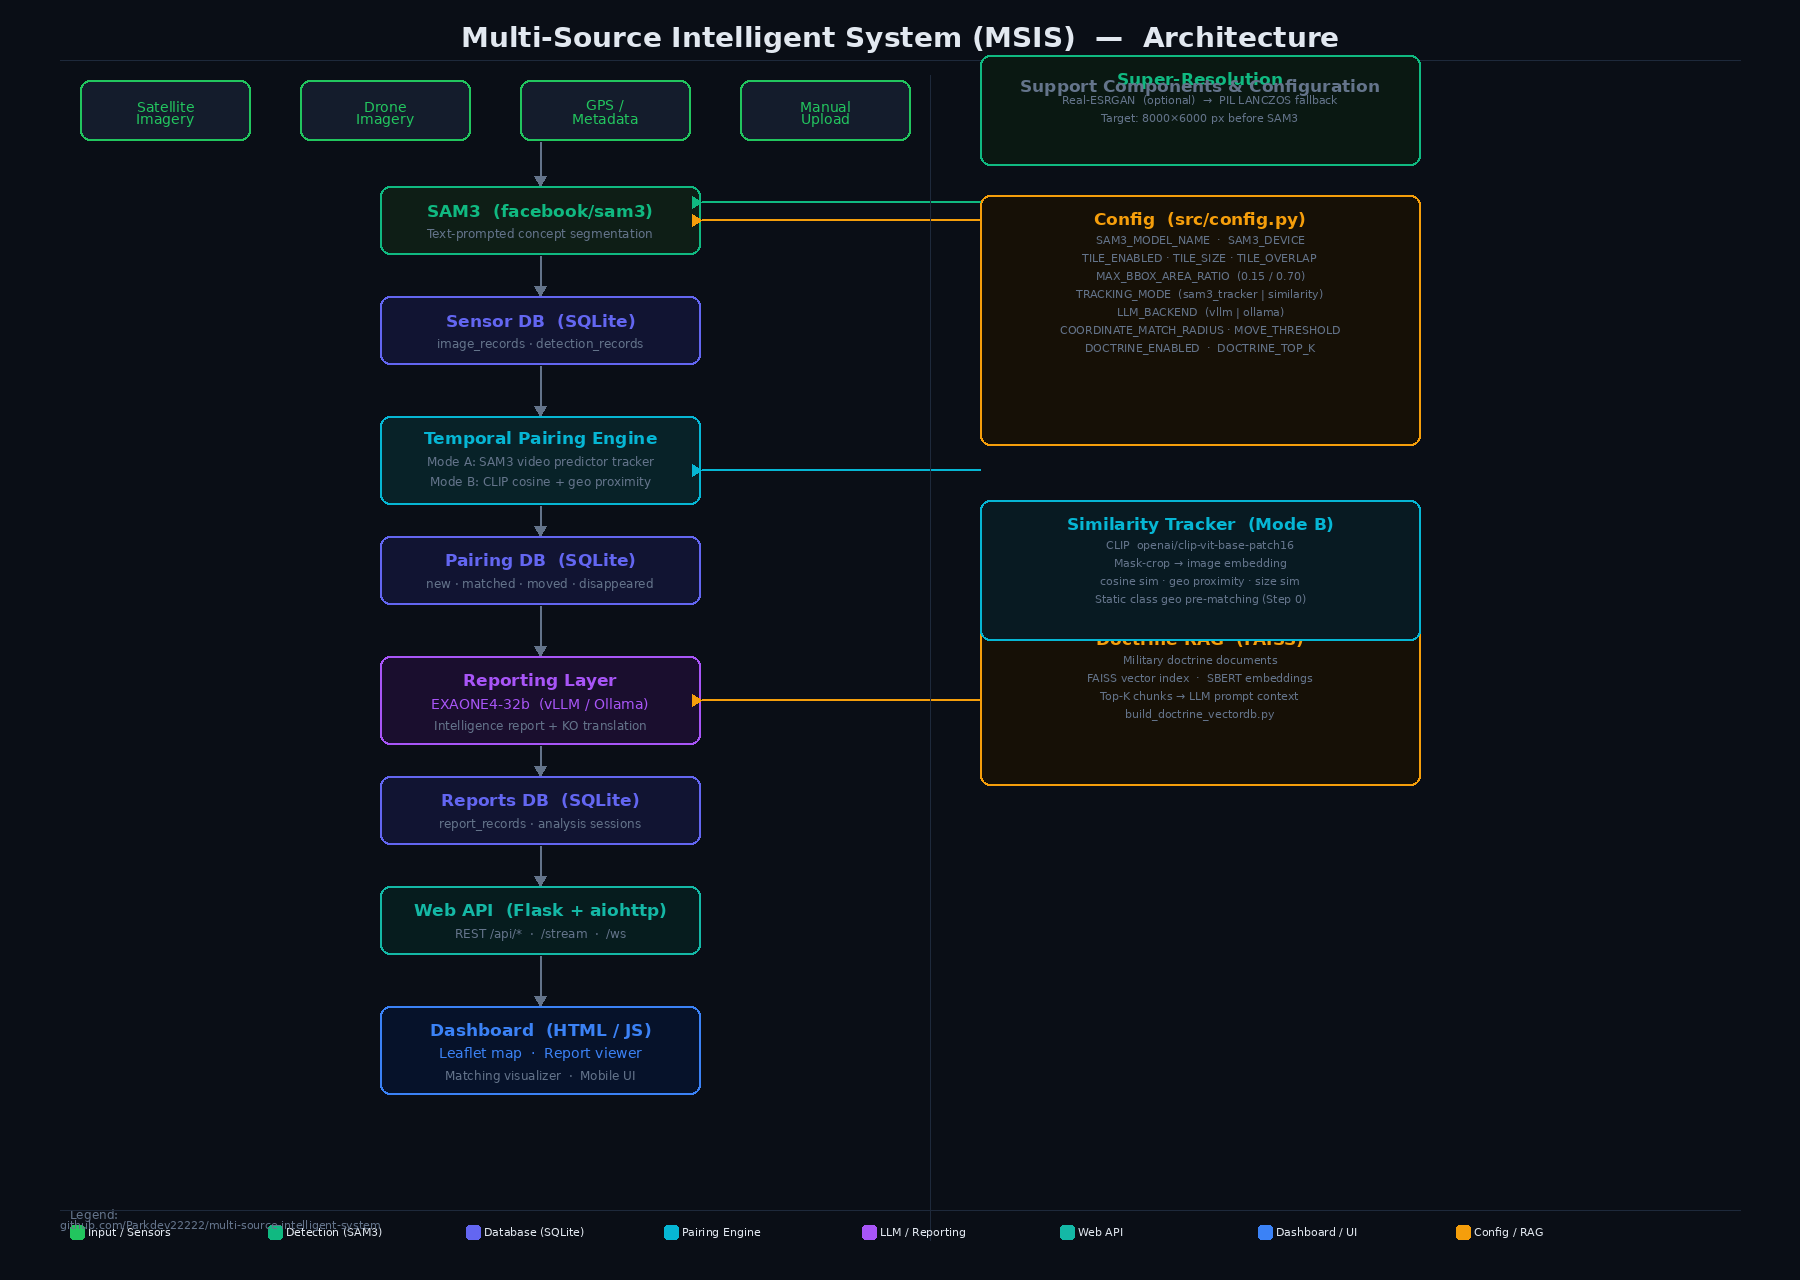
\includegraphics[width=\columnwidth]{../docs/architecture.png}
\caption{Pipeline. Two revisits are segmented independently; detections are
geo-referenced; the learned head matches instances across frames and verifies
the unmatched ones; survivors are written to a persistent spatio-temporal graph
that the report is generated from.}
\label{fig:architecture}
\end{figure}

\subsection{Pipeline}

Two co-registered revisits of a tile enter; a report leaves. An
open-vocabulary segmenter (\DetectorName) proposes object instances in each
frame independently, at three scales, with non-maximum suppression across
scales. Each detection is geo-referenced through an invertible
pixel-to-latitude/longitude transform, so every downstream stage reasons in
world coordinates rather than tile coordinates and observations of the same
place from different tiles or dates coincide.

The pairing head then decides, for candidate detection pairs across the two
frames, which are the same physical object, and for detections left unmatched,
which represent a genuine change. Surviving instances are written into a
persistent spatio-temporal knowledge graph keyed by location, so a
neighbourhood accumulates entity histories across revisits. The report is
generated from that structure rather than from the images.

\subsection{Learned Pairing}

Let $P$ and $C$ be the detections in the past and current frames. Candidate
pairs are formed within a geographic radius. For each candidate we compute
\NPairFeatures{} pair features: CLIP cosine between mask-cropped patches,
geodesic centre distance normalised by the match radius, IoU of the
geo-referenced boxes, log area ratio, aspect difference, both confidences,
class agreement, signed centre offsets, mutual-best-match indicators for CLIP
and geometry, normalised candidate ranks, and candidate densities on both
sides. The rank and density features matter more than they look: they let the
head condition on how contested a match is, which a pairwise similarity alone
cannot express.

For each detection we compute \NUnaryFeatures{} unary features: confidence,
log relative area, aspect, position in the tile, mask fill ratio (a proxy for
segmentation quality), the best geometric and CLIP agreement it finds in the
other frame, the number of overlapping detections there, distance to the tile
edge, and \NCrossFrameFeatures{} cross-frame features described below.

Three small multi-layer perceptrons share a class embedding
(Fig.~\ref{fig:architecture}): $\mathrm{match}$ scores a candidate pair,
$\mathrm{state}$ classifies a matched pair as stationary, moved or modified,
and $\mathrm{verify}$ scores whether an unmatched detection is a genuine change
instance. Each is two hidden layers of width 64 with layer normalisation, GELU
and dropout; features are standardised with statistics fitted on the training
split. The whole head is \HeadParams{} parameters.

Matching is a greedy assignment over $\mathrm{match}$ scores above a threshold;
we also report a variant using the Hungarian algorithm, which changes the
result by less than 0.1 F1. Unmatched detections are kept only if
$\mathrm{verify}$ exceeds its own threshold. Both thresholds are selected on
the validation split and never on test.

\textbf{Supervision is free.} Change-detection benchmarks publish binary change
masks. We convert a mask to instances by connected components, then label a
candidate pair positive when both detections fall outside the change region and
co-locate, and label an unmatched detection positive when it overlaps a
ground-truth change instance. No annotation beyond what the benchmark already
ships is required, which is what makes the head cheap to retrain for a new
sensor or region.

\subsection{Cross-Frame Co-located Evidence}

The dominant failure of any detect-then-pair design is asymmetric detector
recall. If the segmenter misses a building in the past frame and finds it in
the current one, pairing has nothing to pair against and the object is reported
as new construction. The evidence that it was already there is in the past
frame's pixels, not in its detections.

For every detection we therefore crop \emph{the same geographic footprint} from
both frames --- regardless of whether the detector fired in the other frame ---
and compute four quantities: CLIP cosine between the two crops, mean absolute
pixel difference, normalised cross-correlation, and signed edge-density change,
which rises sharply when a roof appears. These are handed to $\mathrm{verify}$
as features rather than compared against a fixed threshold, which is what the
production heuristic did.

Ablating this evidence requires \emph{retraining} without it, not zeroing it at
inference: after standardisation, zero is not a neutral input, so zeroing
measures a broken model rather than the feature's contribution. Retrained
without it, the head loses \EOneCrossFrameGain{} pixel F1 and
\EOneCrossFrameInstGain{} instance F1.

\subsection{Spatio-Temporal Knowledge Graph and Report Generation}

Verified instances are upserted into a graph keyed by geographic location:
entity nodes with observation histories, location nodes, and typed relations
between them. Community detection over the entity graph yields neighbourhood
summaries. On a revisit, an entity is matched to its own history by location,
so the graph accumulates rather than resets.

Report generation is conditioned on progressively more of this structure, which
gives the grounding ladder we ablate in Section~\ref{sec:experiments}:

\begin{itemize}
\item \texttt{template} --- deterministic prose from the change inventory, no
      language model. This is not a hallucination-free condition: it invents no
      sentences but states whatever the detector found, so every detection
      error becomes an unsupported claim. It fixes the error floor our own
      detector imposes.
\item \texttt{vlm\_direct} --- an external baseline: a vision--language model
      shown both images and none of our pipeline.
\item \texttt{llm\_raw} --- a language model over the unaggregated detection
      dump.
\item \texttt{llm\_struct} --- over the aggregated change inventory, isolating
      aggregation.
\item \texttt{llm\_flat\_rag} --- plus top-$k$ retrieved past observations,
      isolating whether \emph{any} history helps.
\item \texttt{llm\_graphrag} --- plus entity histories and community summaries.
\end{itemize}

\texttt{llm\_flat\_rag} is the condition that makes the comparison honest:
without it, a gain from graph grounding could be nothing more than ``retrieval
helps''.

\section{Change-Fact-Score}
\label{sec:cfs}

BLEU rewards phrasing that overlaps the references and is blind to a report
confidently announcing construction that never happened. A monitoring service
is judged on the second thing. We therefore score reports at the level of the
claims they make.

A deterministic rule-based extractor reduces a report to a set of atomic claims
\[
  c = (\textit{direction},\ \textit{object class},\ \textit{count}),
\]
where \textit{direction} $\in$ \{appeared, disappeared, modified, none\}. Each
sentence is scanned for a direction cue, an object class, and a numeral or
quantifier; a sentence with no direction cue makes no claim. An explicit change
claim overrides a co-occurring no-change claim in the same report.

The same extractor is applied to the five human reference captions, and a
reference claim is kept when at least two annotators support it. Ground-truth
counts come from the mask's connected components. Precision and recall of the
predicted claim set against the reference claim set give CFS-P, CFS-R and
CFS-F1. Two further quantities are read directly: ChgAcc, whether the report
agrees with the ground truth on the binary question of whether anything changed
at all, and CountMAE, the absolute error in the number of instances asserted.

Two properties matter for review. First, \textbf{no language model sits inside
the metric}, so the model under evaluation cannot optimise against the judge
and the score does not inherit a judge's failure modes. Second,
\textbf{hallucination rate is not an independent number}: we define it as
$1 - \text{CFS-P}$, so reporting both in one table would give two columns
carrying one measurement. We report CFS-P/R/F1 in tables and quote the
hallucination rate only in prose, where ``one claim in four is unsupported''
reads more directly than a precision.

The metric earns its place on the external baseline. A vision--language model
shown both images scores BLEU-4 \EFourVLMBleu{} --- low, but low BLEU is
routinely explained away as stylistic mismatch. ChgAcc shows what is actually
happening: \EFourVLMChgAcc\%, indistinguishable from chance on whether the
scene changed, while the prose reads fluently. That failure is what the
pipeline exists to avoid, and n-gram overlap alone would not have surfaced it.

\section{Experiments}
\label{sec:experiments}

\subsection{Setup}

Detection uses \DetectorName{} with CLIP embeddings per instance; text
conditions use \LLMName{} and the image-conditioned baseline uses \VLMName,
both served through vLLM. Change detection is evaluated on LEVIR-CD (test, 128
tiles) and WHU-CD (test, 690 pairs); report quality on LEVIR-CC. All timings
are measured on one A100 80GB.

\textbf{Integrity.} Every run asserts and records four properties: train and
test pair identifiers are disjoint; their parent scenes are disjoint, so two
crops of one tile cannot straddle the split; all thresholds are selected on the
validation split, never on test; and prompt style examples, where used, are
drawn only from the training split. The assertions are part of the result
files, not of the prose.

\textbf{Tiers.} Methods trained on a benchmark's own training split and methods
that have never seen it are not competing on equal terms, and printing them in
one block is misleading whichever way the numbers fall. Tables group by tier
and label each group. Our LEVIR-CD result occupies a third position we state
rather than blur: the detector never saw LEVIR-CD, but the pairing head was
trained on its training split from mask-derived labels, so it is not
zero-shot. Section~\ref{ssec:e2} is the zero-shot claim.

\subsection{Change Detection (E1)}

\begin{table}[t]
\centering
\caption{Pixel-level change detection on LEVIR-CD. Baselines are fully supervised; ours is open-vocabulary with a 20k-parameter pairing head.}
\label{tab:levir_cd_pixel}
\setlength{\tabcolsep}{4pt}
\begin{tabular}{lcccc}
\toprule
Method & P & R & F1 & IoU \\
\midrule
\multicolumn{5}{l}{\emph{Trained on this dataset (reference ceiling)}} \\
FC-Siam-Diff~\cite{daudt2018fully} & 89.53 & 83.31 & 86.31 & 75.92 \\
STANet~\cite{chen2020spatial} & 83.81 & 91.00 & 87.26 & 77.40 \\
SNUNet~\cite{fang2021snunet} & 89.18 & 87.17 & 88.16 & 78.83 \\
BIT~\cite{chen2021remote} & 89.24 & 89.37 & 89.31 & 80.68 \\
ChangeFormer~\cite{bandara2022transformer} & 92.05 & 88.80 & 90.40 & 82.48 \\
TinyCD~\cite{codegoni2023tinycd} & -- & -- & 91.05 & 83.57 \\
\midrule
\multicolumn{5}{l}{\emph{Zero-shot / open-vocabulary}} \\
AnyChange (SAM zero-shot)~\cite{zheng2024segment} & 13.70 & 83.00 & 23.40 & -- \\
AnyChange-H + 3-point query~\cite{zheng2024segment} & 28.50 & 81.10 & 42.20 & -- \\
\midrule
\multicolumn{5}{l}{\emph{This work}} \\
geo-only & 14.34 & 64.73 & 23.47 & 13.30 \\
heuristic (production) & 16.08 & 62.67 & 25.59 & 14.67 \\
learned head + greedy & 56.35 & 51.84 & 54.00 & 36.99 \\
learned head, no verifier & 12.49 & 76.66 & 21.48 & 12.03 \\
learned head, no cross-frame & 47.26 & 51.52 & 49.30 & 32.71 \\
\textbf{learned head (ours)} & \textbf{56.22} & \textbf{51.97} & \textbf{54.01} & \textbf{36.99} \\
\bottomrule
\end{tabular}
\end{table}

\begin{table}[t]
\centering
\caption{Instance-level change detection on LEVIR-CD (IoU $\geq$ 0.5).}
\label{tab:levir_cd_instance}
\setlength{\tabcolsep}{4pt}
\begin{tabular}{lccc}
\toprule
Method & P & R & F1 \\
\midrule
\multicolumn{4}{l}{\emph{This work}} \\
geo-only & 32.36 & 39.60 & 35.62 \\
heuristic (production) & 34.11 & 37.48 & 35.72 \\
learned head + greedy & 80.86 & 40.85 & 54.28 \\
learned head, no verifier & 24.34 & 43.62 & 31.25 \\
learned head, no cross-frame & 64.97 & 41.38 & 50.56 \\
\textbf{learned head (ours)} & \textbf{80.79} & \textbf{40.87} & \textbf{54.28} \\
\bottomrule
\end{tabular}
\end{table}


The row worth pointing at is not ours. Geometry-only pairing (\EOneGeoFOne),
the production heuristic (\EOneHeuristicFOne) and AnyChange
(\AnyChangeFOne) all land within two points of each other, at precision 13--16
with high recall. Methods that do not learn to pair converge on the same place
regardless of segmentation quality, and the \HeadParamsRound-parameter head is
what leaves that cluster: \EOnePixelFOne{} pixel F1, $2.3\times$ AnyChange's,
above even its human-assisted three-point setting (\AnyChangeHFOne).

Both ablations are load-bearing. Without the verifier the system scores
\EOneNoVerifierFOne{} --- below geometry-only --- because the head proposes
matches and something has to reject them. Retrained without cross-frame
evidence it loses \EOneCrossFrameGain{} pixel F1.

\subsection{Transfer Without Retraining (E2)}
\label{ssec:e2}

\begin{table}[t]
\centering
\caption{Pixel-level change detection on WHU-CD. Baselines are fully supervised; ours is open-vocabulary with a 20k-parameter pairing head.}
\label{tab:whu_cd_pixel}
\setlength{\tabcolsep}{4pt}
\begin{tabular}{lcccc}
\toprule
Method & P & R & F1 & IoU \\
\midrule
%% TODO fill and verify in baselines.json: FC-Siam-Diff [supervised], BIT [supervised], ChangeFormer [supervised], AnyChange (SAM zero-shot) [zero-shot]
\midrule
\multicolumn{5}{l}{\emph{This work}} \\
geo-only & 23.35 & 42.57 & 30.16 & 17.76 \\
heuristic (production) & 21.73 & 42.98 & 28.86 & 16.87 \\
learned head + greedy & 73.06 & 48.05 & 57.97 & 40.82 \\
learned head, no verifier & 12.13 & 53.50 & 19.78 & 10.98 \\
\textbf{learned head (ours)} & \textbf{72.89} & \textbf{48.05} & \textbf{57.92} & \textbf{40.77} \\
\bottomrule
\end{tabular}
\end{table}

\begin{table}[t]
\centering
\caption{Instance-level change detection on WHU-CD (IoU $\geq$ 0.5).}
\label{tab:whu_cd_instance}
\setlength{\tabcolsep}{4pt}
\begin{tabular}{lccc}
\toprule
Method & P & R & F1 \\
\midrule
\multicolumn{4}{l}{\emph{This work}} \\
geo-only & 4.73 & 55.62 & 8.73 \\
heuristic (production) & 4.93 & 55.93 & 9.06 \\
learned head + greedy & 44.18 & 63.83 & 52.22 \\
learned head, no verifier & 2.51 & 68.90 & 4.85 \\
learned head, no cross-frame & 38.63 & 63.32 & 47.98 \\
\textbf{learned head (ours)} & \textbf{44.18} & \textbf{63.83} & \textbf{52.22} \\
\bottomrule
\end{tabular}
\end{table}


The head is applied to WHU-CD unchanged: no retraining, and the thresholds are
those selected on LEVIR-CD's validation split. It reaches \ETwoPixelFOne{}
pixel F1 against \ETwoHeuristicFOne{} for the heuristic it replaces, and
\ETwoInstFOne{} instance F1 against \ETwoHeuristicInstFOne. The verifier
ablation collapses below geometry-only exactly as in E1.

The instance columns state it more usefully than F1 does. Against \ETwoNGT{}
ground-truth instances the heuristic emits \ETwoHeuristicNPred{} predictions
and ours emits \ETwoNPred: count error falls from \ETwoHeuristicCountMAE{} to
\ETwoCountMAE. For a service that reports how many buildings appeared, that is
the difference between a usable number and noise.

\textbf{This is not evidence that transfer is easier than the source domain.}
WHU-CD test averages \ETwoGTDensity{} ground-truth instances per tile against
LEVIR-CD's \EOneGTDensity, a $38\times$ difference in change density, so
\ETwoPixelFOne{} and \EOnePixelFOne{} are not comparable as difficulties. We
report both densities for that reason.

\subsection{Grounding and Factuality (E3, E4)}

\begin{table}[t]
\centering
\caption{Report factuality by grounding condition (caption style). CFS is claim-level precision/recall against the human references; Hal is the share of generated claims with no ground-truth support.}
\label{tab:factuality_caption}
\setlength{\tabcolsep}{4pt}
\begin{tabular}{lccccc}
\toprule
Method & CFS-P & CFS-R & CFS-F1 & Hal & ChgAcc \\
\midrule
\multicolumn{6}{l}{\emph{This work}} \\
template & 61.55 & 39.60 & 48.20 & 38.45 & 76.46 \\
vlm_direct & 34.97 & 24.03 & 28.49 & 65.03 & 45.78 \\
llm_raw & 55.87 & 38.06 & 45.28 & 44.13 & 70.40 \\
llm_struct & 61.73 & 39.76 & 48.37 & 38.27 & 76.46 \\
llm_flat_rag & 61.96 & 39.85 & 48.51 & 38.04 & 76.57 \\
\textbf{llm_graphrag} & \textbf{61.72} & \textbf{39.70} & \textbf{48.32} & \textbf{38.28} & \textbf{76.52} \\
\bottomrule
\end{tabular}
\end{table}

\begin{table}[t]
\centering
\caption{Change captioning on LEVIR-CC. Baselines are trained on the LEVIR-CC training split; our conditions are zero-shot apart from the pairing head.}
\label{tab:levir_cc_caption}
\setlength{\tabcolsep}{3pt}
\begin{tabular}{lccccc}
\toprule
Method & BLEU-1 & BLEU-4 & METEOR & ROUGE-L & CIDEr-D \\
\midrule
\multicolumn{6}{l}{\emph{Trained on this dataset (reference ceiling)}} \\
DUDA~\cite{park2019robust} & 81.44 & 57.79 & 37.15 & 71.04 & 124.32 \\
MCCFormers-S~\cite{qiu2021describing} & 82.16 & 59.41 & 38.26 & 72.10 & 128.34 \\
MCCFormers-D~\cite{qiu2021describing} & 80.49 & 57.34 & 38.23 & 71.40 & 126.85 \\
RSICCformer~\cite{liu2022remote} & 84.11 & 61.93 & 38.79 & 73.02 & 131.40 \\
Chg2Cap~\cite{chang2024changes} & 86.14 & 64.39 & 40.03 & 75.12 & 136.61 \\
\midrule
\multicolumn{6}{l}{\emph{This work}} \\
\texttt{template} & 50.33 & 26.03 & 51.50 & 47.10 & 25.29 \\
\texttt{vlm\_direct} & 31.85 & 4.51 & 21.71 & 25.27 & 11.47 \\
\texttt{llm\_raw} & 53.02 & 29.15 & 40.66 & 44.72 & 60.11 \\
\texttt{llm\_struct} & 48.09 & 28.15 & 49.90 & 51.49 & 77.77 \\
\texttt{llm\_flat\_rag} & 49.52 & 29.19 & 50.42 & 52.06 & 78.35 \\
\textbf{\texttt{llm\_graphrag}} & \textbf{49.53} & \textbf{29.56} & \textbf{49.81} & \textbf{51.63} & \textbf{78.00} \\
\bottomrule
\end{tabular}
\end{table}


Two results in this table have to be reported rather than buried.

\textbf{The external baseline decides at chance.} \texttt{vlm\_direct} reaches
ChgAcc \EFourVLMChgAcc\% --- it is guessing whether anything changed --- while
producing confident, well-formed prose. CFS-F1 \EFourVLMFOne{} against
\EFourGraphRAGFOne{} for the grounded pipeline.

\textbf{Aggregation is worth \EFourAggGain{} points; retrieval and graph
aggregation on top of it are worth nothing measurable.} Structuring the raw
detection dump into a change inventory moves CFS-F1 from
\EFourRawFOne{} (\texttt{llm\_raw}) to \EFourStructFOne{}
(\texttt{llm\_struct}). Adding top-$k$ retrieval of past observations
(\EFourFlatRagFOne) or replacing it with graph entity and community
aggregation (\EFourGraphRAGFOne) moves it by less than
\EFourLadderSpread{} points, and not consistently in the graph's favour:
over \EFourNCrops{} crops \texttt{llm\_flat\_rag} finishes marginally
ahead. We read the three as indistinguishable rather than ranked.

The reason is structural rather than a shortcoming of the graph. All three
conditions receive the same change inventory for the crop being described, and
CFS scores only claims about \emph{that} crop; retrieved history concerns
\emph{other} crops, so it can move wording but rarely a claim. Measured
directly: of \EFourNCrops{} generations, \EFourTextDiffer{}
(\EFourTextDifferPct\%) differ in text between the three conditions and
only \EFourClaimsDiffer{} (\EFourClaimsDifferPct\%) differ in extracted
claims. A crop-level ladder therefore cannot decide the question it appears to
ask, and reporting the three as an ablation would be presenting noise as a
result. Section~\ref{ssec:e7} asks it at the unit where the answer can differ.

\textbf{Generation adds no measurable factuality over the deterministic
template.} The template states its claims from the same inventory without a
language model and is not separated from the generated conditions on CFS. What
generation adds is prose a subscriber can read, which is a different claim
requiring different evidence, and we do not measure readability here.

\subsection{Pairing Determines Report Factuality (E5)}

E4 varies grounding with pairing fixed; E5 does the reverse. Grounding is
pinned at \texttt{llm\_graphrag} and only the pairing is swapped, so whatever
moves is attributable to pairing. Unlike the graph term, the swapped variable
demonstrably reaches the evidence: every crop receives a different change
inventory.

% generated by paper/make_tables.py -- do not edit
% CLIP + geometry heuristic: results/levir_cc_caption_heuristic_pairing (n=1929, checkpoint=None)
% learned head (ours): results/levir_cc_caption (n=1929, checkpoint=data/checkpoints/pairing_head.pt)
\begin{table}[t]
\centering
\caption{Report factuality under two pairing methods (E5).}
\label{tab:e5_pairing}
\setlength{\tabcolsep}{4pt}
\begin{tabular}{lccccc}
\toprule
Pairing & CFS-P & CFS-R & CFS-F1 & Hal & ChgAcc \\
\midrule
CLIP + geometry heuristic & 34.01 & 36.79 & 35.35 & 65.99 & 65.01 \\
\textbf{learned head (ours)} & \textbf{61.72} & \textbf{39.70} & \textbf{48.32} & \textbf{38.28} & \textbf{76.52} \\
\bottomrule
\end{tabular}
\vspace{1pt}
\parbox{\columnwidth}{\scriptsize\textit{Note:} Grounding is fixed at \texttt{llm\_graphrag}; crops, style examples and the language model are identical across rows. The heuristic has no verifier, so this gap combines matching and suppression; Section~\ref{ssec:ablation} decomposes them for detection.}
\end{table}


Report factuality moves by \EFiveGain{} CFS-F1. Two of every three claims the
heuristic-fed report makes are unsupported (\EFiveHeuristicHal\%), against one
in four (\EFiveLearnedHal\%) for the learned head; ChgAcc rises from
\EFiveHeuristicChgAcc{} to \EFiveLearnedChgAcc. This is the measurement that
connects detection quality to the product: E1 and E2 show the head detects
better, and E5 shows the improvement survives into what the subscriber is
shown. A paper with E1 alone would be asserting that link rather than measuring
it.

\subsection{Neighbourhood-Level Grounding (E7)}
\label{ssec:e7}

At crop level the conditions are nested and the graph term vanishes. At
neighbourhood level they stop being a ladder and become three
\emph{representations} of the same observations --- full concatenation, top-$k$
retrieval, graph aggregate --- and the comparison becomes decidable. One report
is generated per neighbourhood over every crop of the tile the split provides.

% generated by paper/make_tables.py -- do not edit
% source: results/levir_cc_scene (checkpoint=data/checkpoints/pairing_head.pt)
\begin{table}[t]
\centering
\caption{Neighborhood-level grounding (E7): one report per neighborhood, over every crop of a tile the split provides. The conditions are three representations of the same observations, not an additive ladder. $n=218$, 1--16 crops each (mean 8.8; 129 scenes with more than one crop), mean 37.7 ground-truth instances per scene.}
\label{tab:e7_scene}
\setlength{\tabcolsep}{4pt}
\begin{tabular}{lccc}
\toprule
Representation & CFS-F1 & Hal & scene CountMAE \\
\midrule
template (no LLM) & 40.99 & 56.46 & 26.15 \\
full concatenation & 21.02 & 76.58 & 458.46 \\
top-$k$ retrieval & 18.54 & 78.57 & 167.87 \\
graph aggregate & 27.55 & 72.28 & 18.50 \\
\bottomrule
\end{tabular}
\end{table}


\textbf{Counting is where representation decides the outcome, and the margins
are not subtle.} Concatenating every crop's inventory into one prompt produces
a scene count error of \ESevenStructCountMAE{} instances; top-$k$ retrieval,
which drops crops by construction, reaches \ESevenFlatCountMAE; graph
aggregation reaches \ESevenGraphCountMAE. The failure mode of concatenation is
worth naming: handed everything, the language model does not aggregate it, and
the error grows with the number of observations rather than shrinking. Top-$k$
retrieval is better only because it truncates the prompt, and it cannot recover
a count from crops it never retrieved. Aggregating before generation is what
survives.

\textbf{Graph aggregation is the only generated condition that beats the
deterministic template on any axis}, and it does so on the axis this
application cares about: \ESevenGraphCountMAE{} against the template's
\ESevenTemplateCountMAE. On claim-level factuality it leads the other generated
conditions (\ESevenGraphFOne{} against \ESevenStructFOne{} and
\ESevenFlatFOne) but still trails the template (\ESevenTemplateFOne). We
therefore claim that graph aggregation preserves counts better than either
retrieval or concatenation, and that it is what makes generated
neighbourhood-level reports numerically usable --- not that generation improves
factuality overall.

\textbf{Scale is what made this measurable.} An earlier run over
\PilotESevenNScenes{} scenes put graph aggregation \emph{below} plain
concatenation on CFS-F1 (\PilotESevenGraphFOne{} against
\PilotESevenStructFOne). Over \ESevenNScenes{} scenes the ordering reverses and
the counting gap widens by more than an order of magnitude. The two results are
consistent rather than contradictory: with few observations any representation
serves, and the cost of not aggregating appears only once there are enough
observations to lose track of.

\subsection{Deployment Cost (E6)}

\begin{table}[t]
\centering
\caption{Per-tile processing cost on a single NVIDIA A100 80GB. The learned pairing head adds 19781 parameters and 0.70~ms/tile over the hand-tuned heuristic it replaces --- 0.01\% of the pipeline. Segmentation and language generation dominate the budget.}
\label{tab:efficiency}
\begin{tabular}{lrr}
\toprule
Stage & Latency (ms/tile) & Peak GPU (MB) \\
\midrule
SAM3 detection + CLIP (2 frames) & 6099.45 & -- \\
pairing: heuristic (production) & 8.98 & 0 \\
pairing: learned head (ours) & 9.69 & 10 \\
knowledge graph: index + retrieve & 141.56 & 8 \\
report LLM (server:LGAI-EXAONE/EXAONE-4.0-32B@http://127.0.0.1:8005/v1, batched) & 438.29 & 8 \\
\bottomrule
\end{tabular}
\end{table}


Measured over 512 pairs of the same cache the report experiments use.
Segmentation is \ESixDetectShare\% of the per-tile budget. The learned head
costs \ESixHeadMs~ms against \ESixHeuristicMs~ms for the heuristic it replaces
--- \ESixHeadDelta~ms more, \ESixPipelineShare\% of the pipeline. We quote the
difference rather than characterising it, because the two rows it is derived
from are in the table above and a reader can check the subtraction.

The comparison is only meaningful within one cache. The same measurement over
the 8-scene pilot cache gives 1.45~ms, because those crops carry a different
number of detections and both pairing strategies scale with that count; two
runs over the full cache agree to 0.08~ms. A per-tile latency for this stage is
therefore a property of the tile population, not a constant of the method, and
we report it against the population the rest of the paper uses.

\section{Limitations}

\textbf{We do not approach the supervised ceiling.} Models trained on these
benchmarks' training splits reach 86--91 F1 on LEVIR-CD; we reach
\EOnePixelFOne. Our claim is confined to methods that have not been trained on
the benchmark, and to the practitioner's default of prompting a
vision--language model directly.

\textbf{The LEVIR-CD result is not zero-shot.} The detector never saw the
dataset, but the pairing head was trained on its training split from
mask-derived labels. We place it in a third tier rather than inside the
zero-shot group, and Section~\ref{ssec:e2} is what carries the zero-shot claim.

\textbf{The graph's contribution is narrow, and it is a counting result.} At
crop level it is not measurable at all, for the structural reason given in
Section~\ref{sec:experiments}. At neighbourhood level it is decisive on scene
counts and leads the other generated conditions on CFS-F1, but it still trails
the deterministic template there. We claim the counting result and not more.

\textbf{The temporal half of the graph is untested.} The graph is designed to
accumulate entity histories across many revisits, but both benchmarks carry
exactly two timepoints, so what E7 exercises is spatial aggregation over the
crops of one tile, not history over time. The design's main hypothesis is
therefore not evaluated here, and a dataset with more than two acquisitions of
the same area is what would settle it.

\textbf{Generation is not shown to improve factuality.} At crop level the
language-model conditions and the deterministic template are indistinguishable
on CFS, and at neighbourhood level the template leads on CFS-F1. The case for
generation rests on readability and on producing a count a reader can act on,
and we measure only the second.

\textbf{Claim extraction is rule-based.} This is what keeps a language model
out of the metric, but it also means the extractor sees only the direction
cues, object classes and quantifiers it encodes. It will under-count claims in
phrasings it does not cover, and it is tuned to the vocabulary of this domain.

\textbf{Both change-detection benchmarks are building-centric, and both are
aerial rather than satellite.} Generalisation to other change types and to
lower ground sampling distances is untested. The two datasets also differ in
change density by more than an order of magnitude, which is why we report
density alongside F1 rather than comparing the two scores directly.

\section{Conclusion}

A consumer monitoring service is judged on the sentences it sends, so we built
and measured the pipeline accordingly. The component that matters is small: a
\HeadParamsRound-parameter pairing head, supervised for free from masks the
benchmarks already publish, deciding which detections across two revisits are
the same object and which unmatched detections are real change. It lifts
detection from the 23--26 F1 band that every non-learned pairing strategy
occupies to \EOnePixelFOne{} on LEVIR-CD, and it carries that to WHU-CD
unchanged at \ETwoPixelFOne, cutting instance count error to \ETwoCountMAE.

Measuring the reports required a metric with no language model inside it.
Change-Fact-Score reduces a report to atomic claims and checks them against
human references and ground-truth masks; it is what shows that a
vision--language model given both images writes fluently while deciding at
chance whether anything changed. Holding grounding fixed and swapping only the
pairing moves report factuality by \EFiveGain{} points, which is the link
between detection quality and product quality stated as a measurement rather
than an assumption.

The graph earns a narrower claim than the one we set out to make. Its
contribution is unmeasurable at crop level for structural reasons, and at
neighbourhood level it is a counting result: handed every crop of a tile, a
language model's scene count degrades badly
(\ESevenStructCountMAE{} instances of error), while aggregating through the
graph first holds it to \ESevenGraphCountMAE{} --- better than the
deterministic template and an order of magnitude better than either
alternative. What that does not yet test is the temporal half of the design,
because both benchmarks carry two acquisitions and the graph is built to
accumulate across many. A dataset with a real revisit history is the experiment
this work now needs, alongside change types beyond buildings and true satellite
ground sampling distances.


\bibliographystyle{IEEEtran}
\bibliography{refs}

\end{document}
